\documentclass[11pt,a4paper,titlepage]{article}
\usepackage[english, ngerman]{babel}
%\usepackage{bibgerm} % Zum Einbinden einer Bibliothek (wird hier nicht benötigt)
\usepackage[latin1]{inputenc}
\usepackage{graphicx}
\usepackage{epstopdf} % wandelt automatisch eps- in pdf-Dateien um, falls pdf als Ausgabeformat gewählt wird
\usepackage{include/IHA_listing} % einbinden von Quellcode
\setupListingMatlab % lade Setup für Matlab Quellcode, Parameter können in der *.sty file geändert werden ;)
\usepackage[top=3cm, bottom=2.7cm, left=3cm, right=3cm]{geometry} % Package zum einfachen Einstellen des Seitenlayouts
\usepackage{amsmath} % Package zum Einbinden von Formeln etc.
\usepackage{subfigure}
\usepackage{placeins}
\usepackage{latexsym}
\usepackage{amsfonts}
\usepackage{amssymb}	
\usepackage{fancyhdr}
\usepackage{lastpage}
\usepackage[ngerman, num]{isodate}
\usepackage{marvosym}
\usepackage{eurosym}
\usepackage{url}
\usepackage{wrapfig}
\usepackage{xcolor}
\usepackage{tcolorbox}
\usepackage{hyperref}
\usepackage{tabularx}

\parindent0mm
%\usepackage[protrusion=true,expansion=true]{microtype}
%\usepackage[final]{microtype}
%\usepackage{fontspec}
\usepackage{cmbright}


\usepackage{listings}

\usepackage{color}
\definecolor{gray}{rgb}{0.4,0.4,0.4}
\definecolor{darkblue}{rgb}{0.0,0.0,0.6}
\definecolor{cyan}{rgb}{0.0,0.6,0.6}

\lstset{
  basicstyle=\ttfamily,
  columns=fullflexible,
  showstringspaces=false,
  commentstyle=\color{gray}\upshape,
	numbers=none
}

\lstdefinelanguage{XML}
{
  morestring=[b]",
  morestring=[s]{>}{<},
  morecomment=[s]{<?}{?>},
  stringstyle=\color{black},
  identifierstyle=\color{darkblue},
  keywordstyle=\color{cyan},
  morekeywords={xmlns,version,type}% list your attributes here
}


\tcbset{
    frame code={}
    %center title,
    left=2pt,
    right=0pt,
    top=2pt,
    bottom=0pt,
    %colback=gray!70,
    %%colframe=white,
    %%width=\dimexpr\textwidth\relax,
    enlarge left by=0mm,
    %boxsep=5pt,
    arc=0pt,outer arc=0pt,
    }
\tcbset{before upper={\parindent0em}}

\newcommand{\titleFull}{IHAB-rl Mobile Software}
\renewcommand{\title}{IHAB-rl Mobile Software}
\newcommand{\Institute}{Institute of Hearing Technology and Audiology, Oldenburg}
\newcommand{\version}{v1.5}
%
\pagestyle{fancy}
\lhead{\footnotesize \parbox{11cm}{\Institute} }
\rhead{\footnotesize \sffamily \title\ \thepage\ / \pageref{LastPage}}
\lfoot{\footnotesize \parbox{11cm}{Contact: \Letter\ ulrik.kowalk@jade-hs.de} }
\cfoot{}
\rfoot{\footnotesize \sffamily \title\ \thepage\ / \pageref{LastPage}}
\renewcommand{\footrulewidth}{0.4pt}

%
\begin{document} 
 \selectlanguage{english}
\pagestyle{empty}

\sffamily
\mdseries


\textcolor[rgb]{1,1,1}{.}
	\vspace{3cm}
	\begin{center}
	
	\begin{figure}[h]
		\centering
			
\includegraphics[width=0.30\textwidth]{images/Logo_shadow.jpg}
	\end{figure}
	\vspace{3cm}
	\Huge
	\titleFull \ \version
	\normalsize
	\\
	\vspace{1cm}
	Documentation\\
	\vspace{1cm}
	Last updated: \today\\
	\vspace{1cm}
	Source: \url{https://github.com/IHAB-RL/IHAB_MobileSoftware.git}
	\vfill
	\end{center}

%
%\cfoot{}
\clearpage

\tableofcontents

\clearpage

\setcounter{page}{1}
\pagestyle{fancy}

\section{Introduction}

The application you have obtained is a version of the IHAB EMA system. For standalone use no additional equipment will be required except for a computer to facilitate installation and data transfer. The software has been tested on the following devices:
\begin{itemize}
	\item LG Electronics Nexus 5 (Android 5.1 \& 6.0.1)
	\item Motorola XT1032 (Androd 5.1)
	\item Motorola Moto G2  (Android 6.0)
	\item Motorola Moto G8+ (Android 9)
	\item Lenovo TB2 X30F (Android 6.0.1)
	\item Nokia 7 Plus (Android 10)
	\item ...
\end{itemize}

The application is still undergoing development. Please feel free to report bugs or contact us in case of difficulties during installation or usage. The given directions in the operating system settings may vary between devices.


\section{Installation}


\subsection{Requirements}

The device should be reset to its operating system default (\textit{Settings}$\rightarrow$\textit{Backup\&reset}$\rightarrow$\textit{Factory data reset}) prior to the installation. All accounts (\textit{Settings}$\rightarrow$\textit{Accounts}) as well as device administrators (\textit{Settings}$\rightarrow$\textit{Security}$\rightarrow$\textit{Device administrators}) need to be removed, too. On an average size display, the font size should be set to \textit{Large} (\textit{Settings}$\rightarrow$\textit{Display}$\rightarrow$\textit{Font size}). Required for the installation are:

\begin{itemize}
	\item USB connection between smartphone and computer
	\item Free software \textit{ADB} (Android Debug Bridge), e.g. ``Minimal ADB and Fastboot''
	\item IHAB mobile .apk installation file
	\item Questionnaire .xml file
	\item Helpful: free Android file manager, e.g. \href{https://total-commander.de.uptodown.com/android}{``Total Commander''} installed on the device
\end{itemize}


\subsection{Installation steps}

\begin{enumerate}

\vspace{0.5cm}

	\item Install ADB on the computer and add it to the system path.\\
	 
	\item Enable the developer options on the smartphone. How to do this might vary from model to model. The usual procedure is by opening \textit{Settings$\rightarrow$About phone}. At the bottom is an entry showing the \textit{Build number}. This needs to be clicked 7 times until a message appears. If not, please consult the search engine of your choice.\\
	
	\item Go to \textit{Settings}$\rightarrow$\textit{Developer options} and enable \textit{USB Debugging}.\\
	
	\item Connect the phone to the computer and allow debugging via the dialogue on the phone.\\
	
	\item The next step is to establish a working connection between the smartphone and the computer. In order to check for a connection, open a console and type\\
	\\
	\colorbox{black!10}{\texttt{adb devices}}.\\
	\\
	If everything is okay, ADB should find a device. If not, check your connection. In case the computer does not understand the command, ADB needs to be added to the system path.\\
	
	\item Now that a connection has been verified, navigate via the console to the directory that holds the .apk file and input\\
	\\
	\colorbox{black!10}{\texttt{adb install IHAB\_Mobile.apk}}.\\
	\\
	This will install the application. In case a previous version of the application is already installed, type\\
	\\
	\colorbox{black!10}{\texttt{adb install-r IHAB\_Mobile.apk}}.\\
	
	\item In order to make the application a device owner, which is needed for it to run as a dedicated device, type\\
	\\
	\colorbox{black!10}{\texttt{adb shell dpm set-device-owner com.fragtest.android.pa/.AdminReceiver}}.\\
	
	\item To keep any information from popping up and confusing the user, input\\
	\\
	\colorbox{black!10}{\texttt{adb shell appops set android TOAST\_WINDOW deny}}.\\
	
	\item In the application settings \textit{Settings}$\rightarrow$\textit{Apps}$\rightarrow$\textit{IHAB} you need to enable all permissions (Audio input, Memory). This could also be done within the application but it is much simpler to do it upfront.\\
	
	\item On opening, the application will eventually crash because no questionnaire file is present (however, this step is necessary to build the file system). To copy the questionnaire .xml file to its directory on the smartphone, please enter the following command from the directory that holds the .xml file:\\
	\\
	\colorbox{black!10}{\texttt{adb push [questionnaire file name] sdcard/ihab/quest}}\\
	
	
	\newpage
	
	
	\item Restart the phone by entering\\ 
	\\
	\colorbox{black!10}{\texttt{adb reboot}}.\\
\end{enumerate}


\section{Using the application}\label{sec_usage}


\subsection{General purpose}

\begin{wrapfigure}{r}{5cm}
\vspace{-0.5cm}
		\centering
			\begin{minipage}{0.30\textwidth}
			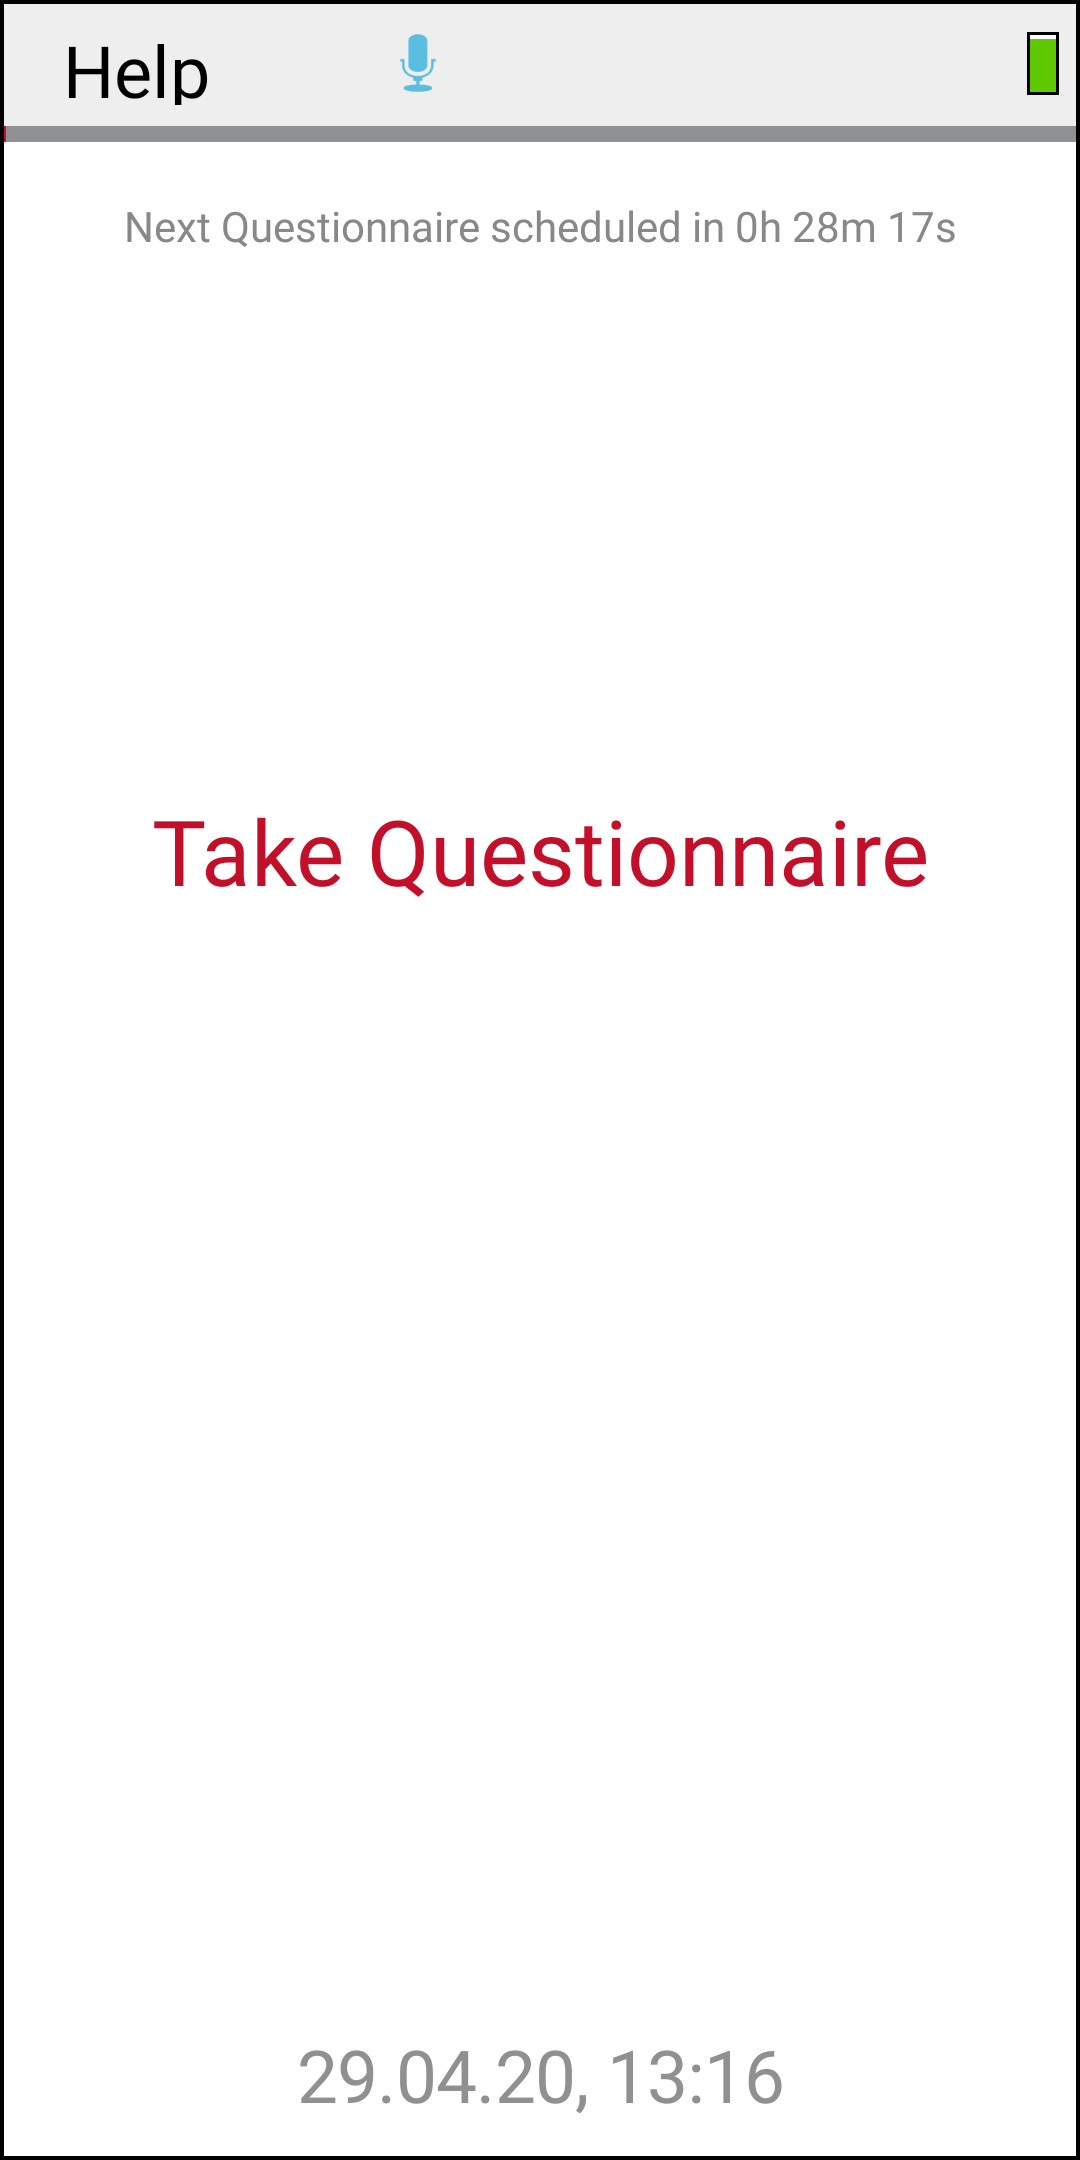
\includegraphics[width=1.00\textwidth]{images/screen_menu_box.png}
			\label{fig:menu}
			\end{minipage}
	\end{wrapfigure}

If the installation was successful, the smartphone now runs as a dedicated device (or kiosk device), meaning that the user cannot leave the application or make alterations to the operating system. Most buttons are disabled or limited to specific use -- including the power button which will only restart the device after a long push.\\
\\
The menu view (see figure on the right) of the application features a bar at the top with a \textit{Help} button, providing a general explanation of the main answer formats. Next to it is a microphone symbol that will change its color according to the type of data input (see \ref{sub:operationmode}). On the right hand side is a battery symbol displaying the current state of charge.\\
\\
The center of the screen features the "Take Questionnaire" button (in case of no major errors present) which can be used to manually start a questionnaire at any given time. Above it is a display of the time until the next questionnaire notification is triggered. If a questionnaire is prompted the font size increases, accompanied by vibrating alert.


\subsection{Experimenter Mode}\label{sub:experimenter}

When testing a new questionnaire, it is helpful to disable the Kiosk mode. The easiest way is via the \textit{Experimenter mode}, which can be unlocked by copying a specific file to the main application folder (\textit{IHAB}). The file may be empty and must be named ``config'' without a formatted ending. To enter the in-app preferences menu, simply hold down the ``HELP'' button in the top left corner for 5 seconds. Inside the preferences, you are free to disable the Kiosk mode as well as change other settings. This will also provide a way to exit a questionnaire by clicking the ``IHAB'' logo in the top left corner. In order to ensure that each questionnaire is answered by the subject, switching off the experimenter mode during an experiment is advisable.


\newpage


\subsection{Operation Modes}\label{sub:operationmode}

The IHAB application offers 6 different modes of operation which are indicated by the color of the microphone symbol at the top center of the screen. If no objective data connection can be established (not needed in Standalone mode), the symbol is gray 
\includegraphics[width=0.02\textwidth]{images/mic_gray.png}. The mode is selected via the preferences menu.

\begin{center}
	\begin{tcolorbox}[colback=black!10!white,colframe=black!50!white, boxsep=1pt,left=4pt,right=4pt,top=4pt,bottom=2pt]
		\begin{tabularx}{\textwidth}{llX} 
		STANDALONE & 
\includegraphics[width=0.02\textwidth]{images/mic_airplaneblue.png} & Application is used for questionnaire purposes only, no additional device needed.\\
		\\
		INTERNAL MIC & 
\includegraphics[width=0.02\textwidth]{images/mic_orange.png} & Objective data is extracted using the internal microphone or the input channel primarily selected by the smartphone.\\
		\\
		USB & 
\includegraphics[width=0.02\textwidth]{images/mic_jadered.png} & Audio data is obtained from a USB audio input device.\\
		\\
		A2DP & 
\includegraphics[width=0.02\textwidth]{images/mic_green.png} & Bluetooth connection using the A2DP protocol. Since this type of connection requires a specialized operating system, it is only available on an LG Nexus 5.\\
		\\
		RFCOMM & 
\includegraphics[width=0.02\textwidth]{images/mic_violet.png} & Bluetooth connection using the RFCOMM protocol using the TGM first generation bluetooth device.\\
		\\
		PHANTOM & 
\includegraphics[width=0.02\textwidth]{images/mic_darkblue.png} & Bluetooth connection using the RFCOMM protocol using the TGM second generation bluetooth device.
		\end{tabularx}
	\end{tcolorbox}
\end{center}

In case of a bluetooth connection, the device must be paired prior to starting the application via the bluetooth settings of the smartphone or tablet computer. This is achieved by \textit{Settings}$\rightarrow$\textit{Connected Devices}$\rightarrow$\textit{Pair new device}.


\subsection{Languages}

The application currently supports English and German. Language settings are adjusted automatically.


\subsection{Log}


A log file named ``\textit{Log2.txt}''is created in the main directory that includes information which can be used to understand and retrace the behavior of the application. 


\section{Compilation of a questionnaire}


\subsection{General outline}

The questionnaires are generated on the basis of .xml files which can be altered to suit the needs of the experiment. Generally it is a good idea to start from an existing file and make changes, testing them regularly on the smartphone in order to guarantee errorless functionality. In case of formal mistakes (e.g. missing brackets or typos within tags) the application might crash. 


\subsection{Location of questionnaire files}

Questionnaire files are placed in the \textit{quest} folder located in the main directory. The application will automatically sort all questionnaire files alphabetically and pick the uppermost. If you would like to use a specific questionnaire, you can choose manually from the preferences menu (see \ref{sub:experimenter}), but we recommend placing only a single file in the \textit{quest} folder in order to avoid confusion. 


\subsection{Head}

The head consists of two lines that must not be changed, but may become obsolete in future releases.

\begin{center}
\begin{tcolorbox}[colback=black!10!white,colframe=black!50!white, boxsep=1pt,left=4pt,right=4pt,top=4pt,bottom=2pt]
\texttt{<?xml version="1.0" encoding="utf-8"?>\\
<mobiquest>}
\end{tcolorbox}
\end{center}


\subsection{Timer}

Two different timer settings exist: \textit{interval} and \textit{fixed schedule}. When choosing interval, a \texttt{mean} and \texttt{deviation} value can be set. The application generates a random interval true to a uniform distribution within the given limits (mean$\pm$deviation). This can be beneficial in order to avoid sampling artifacts, e.g. suggesting a questionnaire every 60 minutes to someone who is always listening to the news at that time. If the scheduling interval should not be random, a deviation value of "0" is set. The timer is re-initiated after a questionnaire has been finalized.

\begin{center}
\begin{tcolorbox}[colback=black!10!white,colframe=black!50!white, boxsep=1pt,left=4pt,right=4pt,top=4pt,bottom=2pt]
\texttt{<timer mean="1800" deviation="300"></timer>}
\end{tcolorbox}
\end{center}

If it is desired to suggest a questionnaire at specific times during the day, the \texttt{date} value must be set. The value is entered in form of a String, meaning a time within quotation marks, e.g. "13:47". The system uses the 24h format HH:mm and multiple dates can be entered by concatenating times with a semicolon, e.g. "12:15;17:21;14:41". Times are sorted automatically by the application. 

\begin{center}
\begin{tcolorbox}[colback=black!10!white,colframe=black!50!white, boxsep=1pt,left=4pt,right=4pt,top=4pt,bottom=2pt]
\texttt{<timer date="12:15;13:13;14:41;17:21;08:10;08:12"></timer>}
\end{tcolorbox}
\end{center}


\subsection{Title}

The title tag can be set to personal taste and is formally needed but does not appear in the output result files.

\begin{center}
\begin{tcolorbox}[colback=black!10!white,colframe=black!50!white, boxsep=1pt,left=4pt,right=4pt,top=4pt,bottom=2pt]
\texttt{<title>\\
\hspace*{0.5cm}<text>Exemplary Questionnaire</text>\\
</title>}
\end{tcolorbox}
\end{center}


\subsection{Questions}

A question consists of an opening \texttt{question} tag including some properties, e.g. id, type, and filter. Then follows the label -- the actual question. After that usually comes a suite of answer options, which are defined by a unique \texttt{option id}. Although there are no restrictions, it has proven useful in practice to combine \texttt{question id} and \# of the answer using an underscore (the underscore is omitted internally) as question ID. The question ID serves as a unique question identifier and the \texttt{type} sets the answer format. There are seven different formats available.


\subsubsection{Single Choice: Radio buttons}

Radio buttons are established as single choice option symbols, meaning that only one option can be selected at the same time.

\begin{center}
\hspace{-1.1cm}
	\begin{tabular}{p{0.68\textwidth} p{0.25\textwidth}} 
		\raisebox{-\totalheight}{
		\begin{tcolorbox}[colback=black!10!white,colframe=black!50!white, boxsep=1pt,left=4pt,right=4pt,top=4pt,bottom=2pt]
		\texttt{\noindent
					$<$question id="10101" type="radio"$>$\newline
					\hspace*{0.5cm}$<$\textbf{label}$>$\newline
					\hspace*{1cm}$<$text$>$Which record is the best?$<$/text$>$\newline
					\hspace*{0.5cm}$<$/\textbf{label}$>$\newline
					\hspace*{0.5cm}$<$\textbf{option} id="10101\_01"$>$\newline
					\hspace*{1cm}$<$text$>$Dark side of the moon$<$/text$>$\newline
					\hspace*{0.5cm}$<$/\textbf{option}$>$\newline
					\hspace*{0.5cm}$<$\textbf{option} id="10101\_02"$>$\newline
					\hspace*{1cm}$<$text$>$Grand Tour$<$/text$>$\newline
					\hspace*{0.5cm}$<$/\textbf{option}$>$\newline
					\hspace*{0.5cm}$<$\textbf{option} id="10101\_03"$>$\newline
					\hspace*{1cm}$<$text$>$Foxtrot$<$/text$>$\newline
					\hspace*{0.5cm}$<$/\textbf{option}$>$\newline
					$<$/\textbf{question}$>$
					}
			\end{tcolorbox} 
		}
		&
		\vspace{-0.29cm}
		\raisebox{-\totalheight}{
			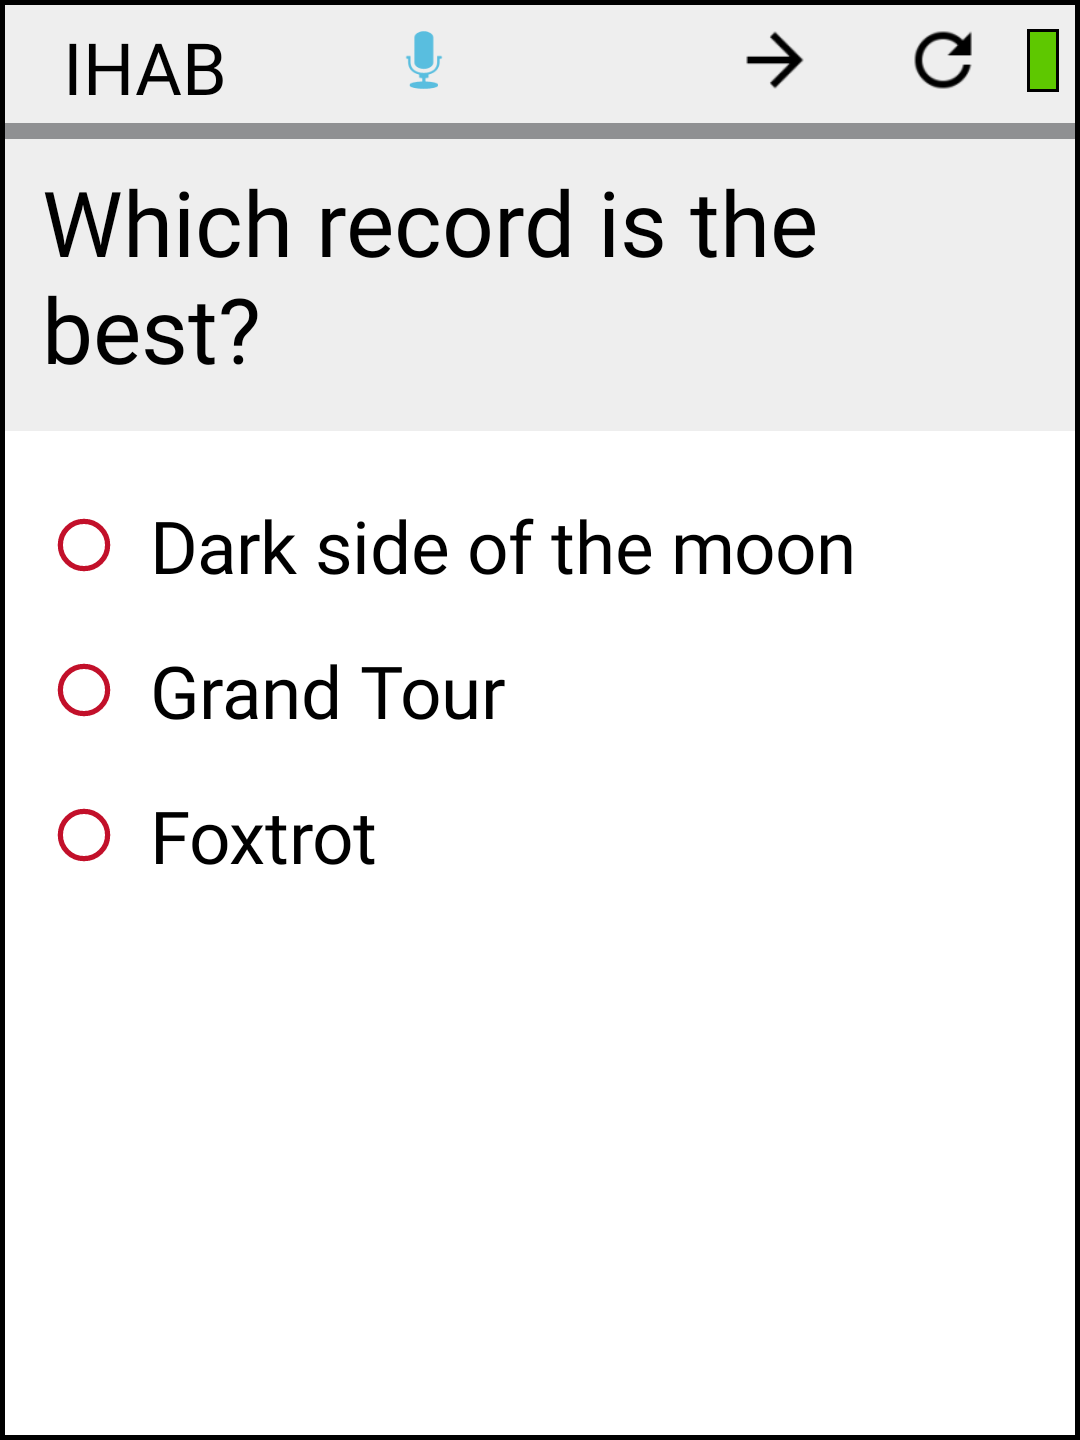
\includegraphics[width=0.30\textwidth]{images/screen_radio_crop_box.png}
		}
	\end{tabular}\\
\end{center}


\subsubsection{Multiple Choice: Checkboxes}

Checkboxes give the user the impression of a list from which multiple items can be selected at the same time. Customized within-list logic can be implemented as described in \ref{subsec:goupingandexclusivity}. 

\begin{center}
\hspace{-1.1cm}
	\begin{tabular}{p{0.68\textwidth} p{0.25\textwidth}} 
		\raisebox{-\totalheight}{
		\begin{tcolorbox}[colback=black!10!white,colframe=black!50!white, boxsep=1pt,left=4pt,right=4pt,top=4pt,bottom=2pt]
		\texttt{\noindent
				$<$question id="10102" type="checkbox"$>$\newline
				\hspace*{0.5cm}$<$label$>$\newline
				\hspace*{1.0cm}$<$text$>$Please select one or more.$<$/text$>$\newline
				\hspace*{0.5cm}$<$/label$>$\newline
				\hspace*{0.5cm}$<$option id="10102\_01"$>$\newline
				\hspace*{1.0cm}$<$text>Red$<$/text$>$\newline
				\hspace*{0.5cm}$<$/option$>$\newline
				\hspace*{0.5cm}$<$option id="10102\_02"$>$\newline
				\hspace*{1.0cm}$<$text$>$Green$<$/text$>$\newline
				\hspace*{0.5cm}$<$/option$>$\newline
				\hspace*{0.5cm}$<$option id="10102\_03"$>$\newline
				\hspace*{1.0cm}$<$text$>$Blue$<$/text$>$\newline
				\hspace*{0.5cm}$<$/option$>$\newline
				</question>
				}
		\end{tcolorbox} 
		}
		&
		\vspace{-0.29cm}
		\raisebox{-\totalheight}{
			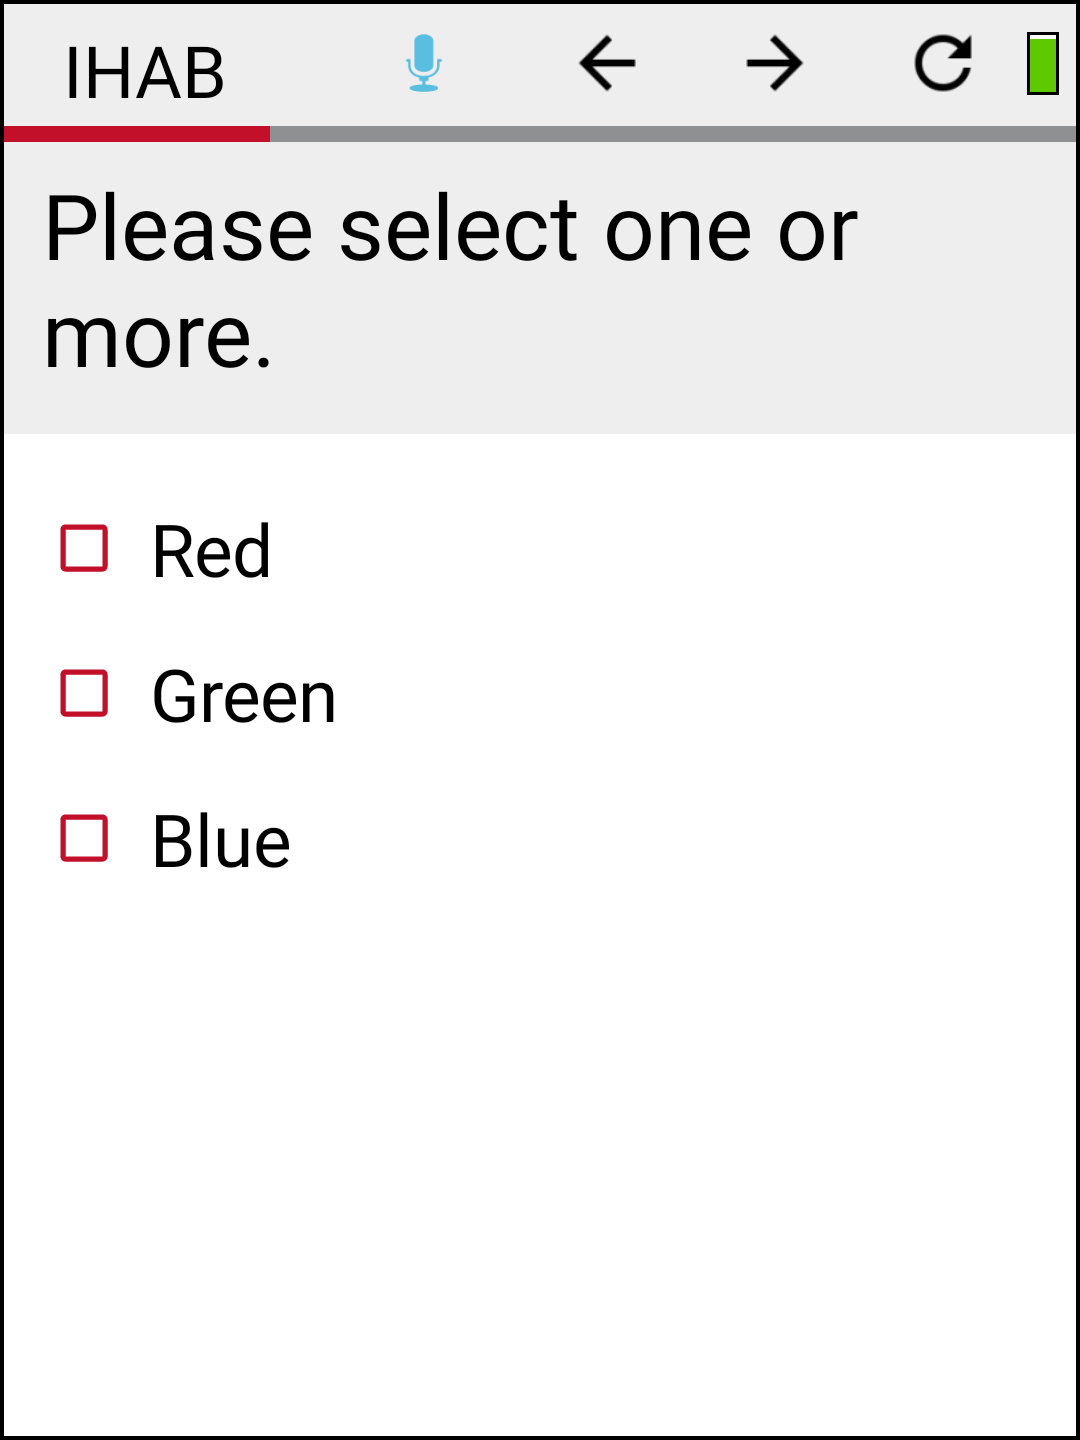
\includegraphics[width=0.30\textwidth]{images/screen_checkbox_crop_box.png}
		}
	\end{tabular}\\
\end{center}


\newpage


\subsubsection{Emojis}  

Emojis yield a swift and intuitive way of assessing the emotional state of a subject. The application comes with five built-in emojis, which are called directly via their file names as shown below. 

\begin{center}
\hspace{-1.1cm}
	\begin{tabular}{p{0.68\textwidth} p{0.25\textwidth}} 
		\raisebox{-\totalheight}{
		\begin{tcolorbox}[colback=black!10!white,colframe=black!50!white, boxsep=1pt,left=4pt,right=4pt,top=4pt,bottom=2pt]
		\texttt{\noindent
			$<$question id="10103" type="emoji"$>$\newline
			\hspace*{0.5cm}$<$label$>$\newline
			\hspace*{1.0cm}$<$text$>$How are you feeling?$<$/text$>$\newline
			\hspace*{0.5cm}$<$/label$>$\newline
			\hspace*{0.5cm}$<$option id="10103\_01"$>$\newline
			\hspace*{1.0cm}$<$text$>$emoji\_happy2$<$/text$>$\newline
			\hspace*{0.5cm}$<$/option$>$\newline
			\hspace*{0.5cm}$<$option id="10103\_02"$>$\newline
			\hspace*{1.0cm}$<$text$>$emoji\_happy1$<$/text$>$\newline
			\hspace*{0.5cm}$<$/option$>$\newline
			\hspace*{0.5cm}$<$option id="10103\_03"$>$\newline
			\hspace*{1.0cm}$<$text$>$emoji\_neutral$<$/text$>$\newline
			\hspace*{0.5cm}$<$/option$>$\newline
			\hspace*{0.5cm}$<$option id="10103\_04"$>$\newline
			\hspace*{1.0cm}$<$text$>$emoji\_sad1$<$/text$>$\newline
			\hspace*{0.5cm}$<$/option$>$\newline
			\hspace*{0.5cm}$<$option id="10103\_05"$>$\newline
			\hspace*{1.0cm}$<$text$>$emoji\_sad2$<$/text$>$\newline
			\hspace*{0.5cm}$<$/option$>$\newline
			$<$/question$>$
			}
		\end{tcolorbox} 
		}
		&
		\vspace{-0.29cm}
		\raisebox{-\totalheight}{
			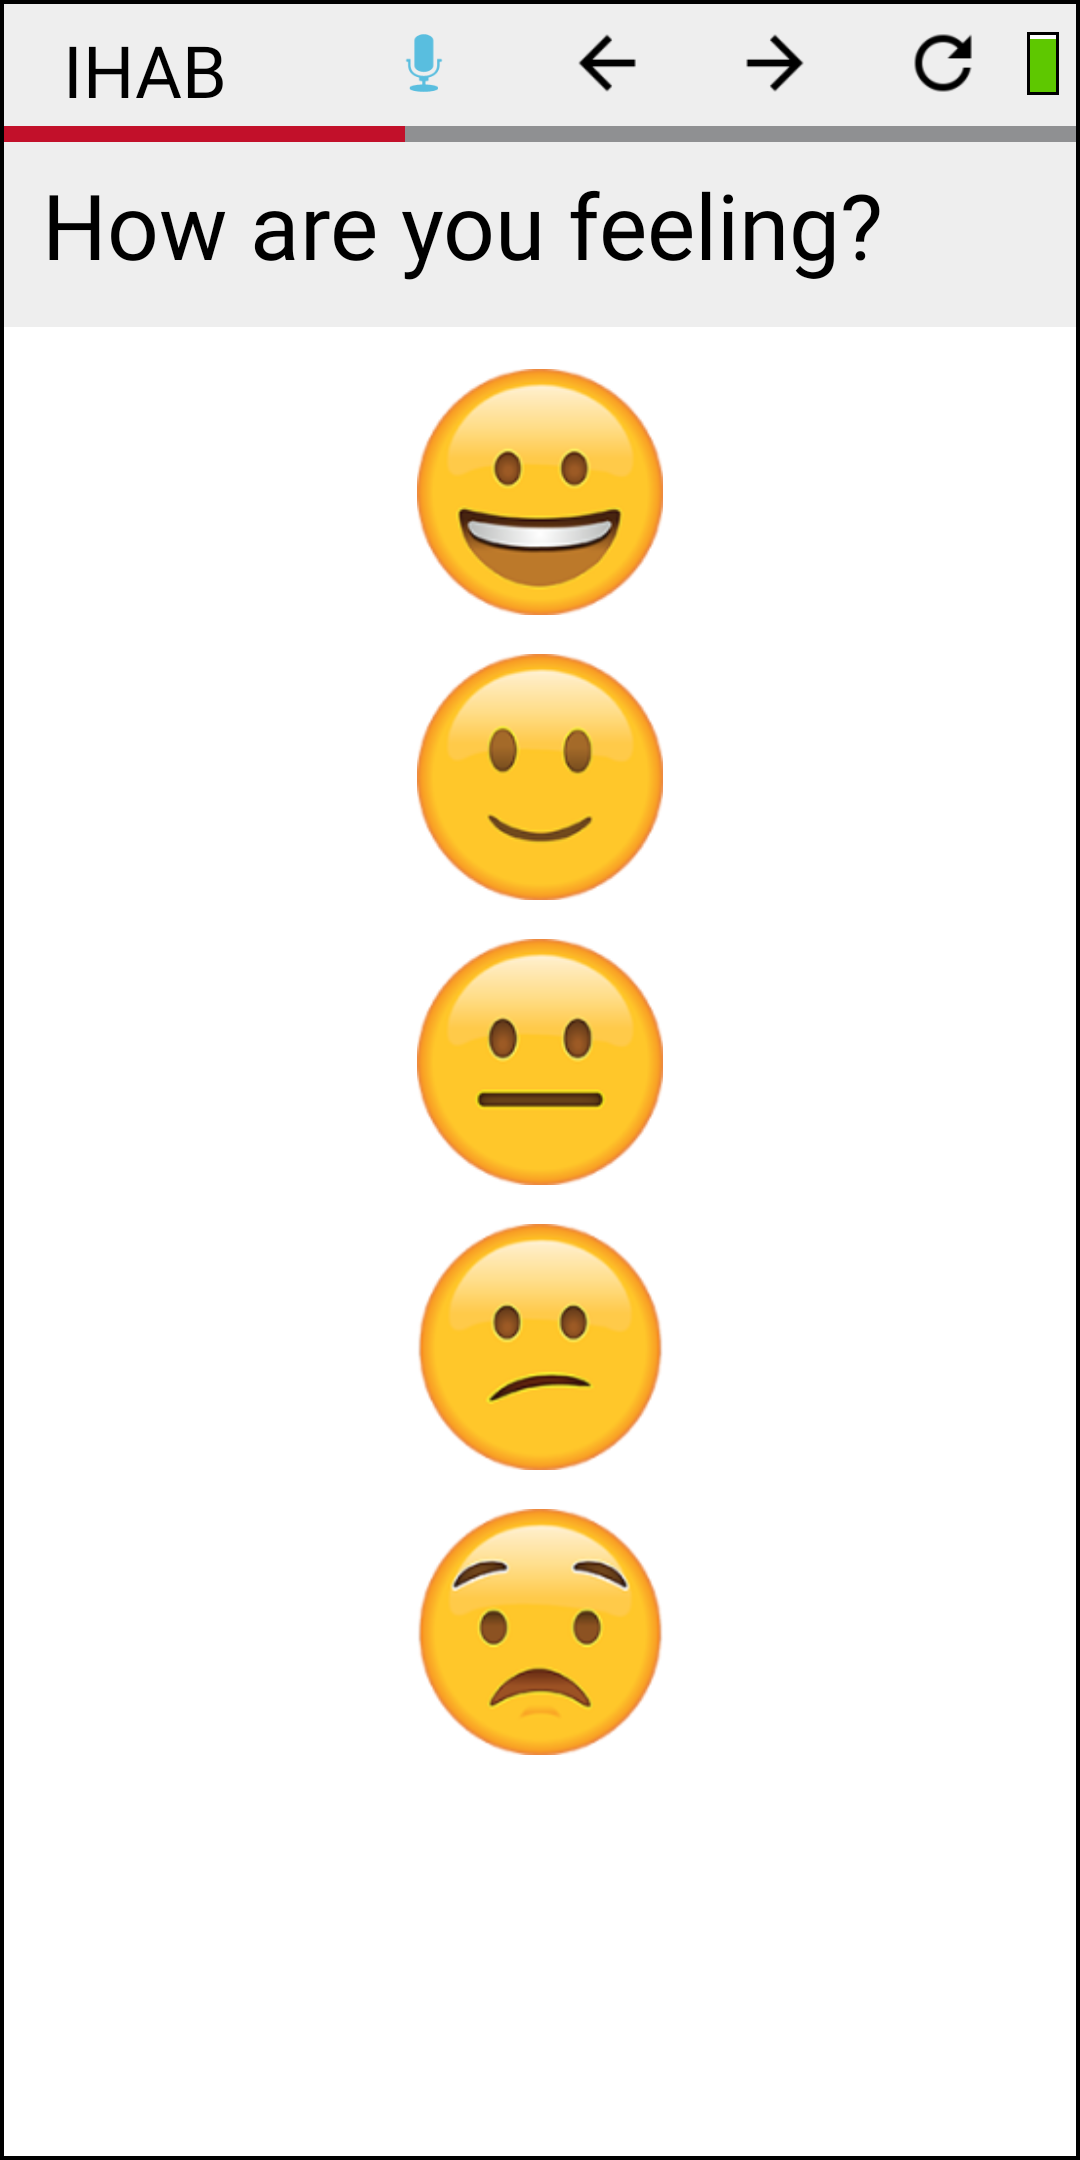
\includegraphics[width=0.30\textwidth]{images/screen_emoji_box.png}
		}
	\end{tabular}\\
\end{center}


\subsubsection{Text}

Sometimes the best way of assessing a situation is via a short text entered by the user. 

\begin{center}
\hspace{-1.1cm}
	\begin{tabular}{p{0.68\textwidth} p{0.25\textwidth}} 
		\raisebox{-\totalheight}{
		\begin{tcolorbox}[colback=black!10!white,colframe=black!50!white, boxsep=1pt,left=4pt,right=4pt,top=4pt,bottom=2pt]
		\texttt{\noindent
			$<$question id="10104" type="text"$>$\newline
			\hspace*{0.5cm}$<$label$>$\newline
			\hspace*{1.0cm}$<$text$>$Please enter text.$<$/text$>$\newline
			\hspace*{0.5cm}$<$/label$>$\newline
			$<$/question$>$
			}
		\end{tcolorbox} 
		}
		&
		\vspace{-0.29cm}
		\raisebox{-\totalheight}{
			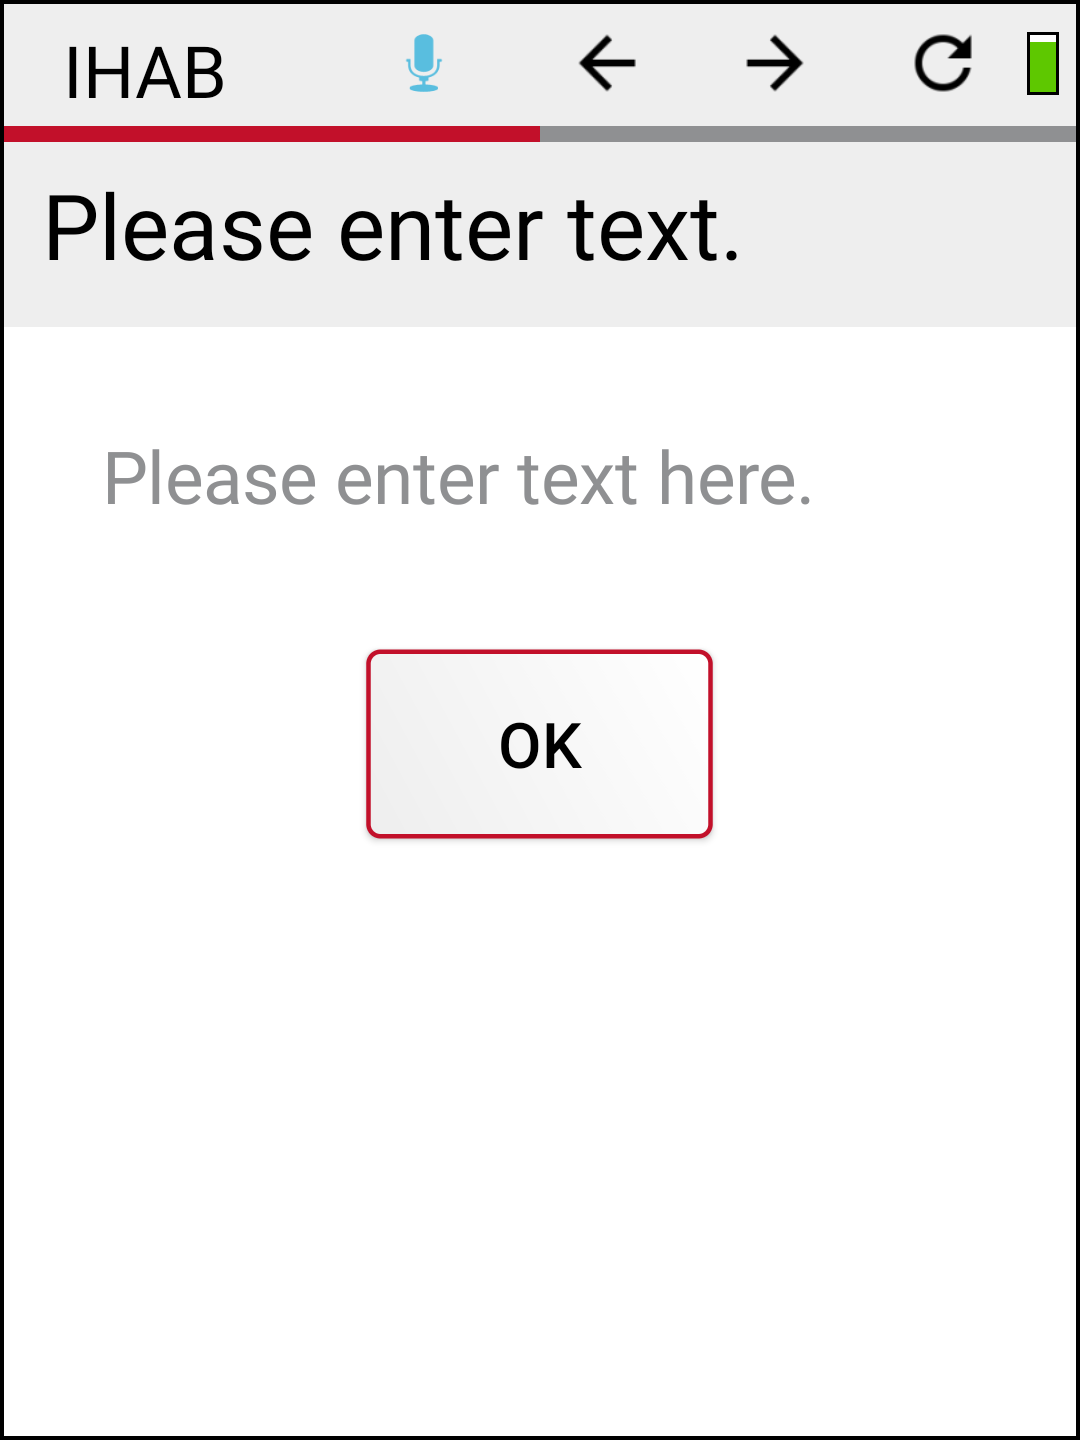
\includegraphics[width=0.30\textwidth]{images/screen_text_crop_box.png}
		}
	\end{tabular}\\
\end{center}


\subsubsection{Fixed Slider}

Fixed sliders technically do no offer a different choice than radio buttons, but they can be helpful when the answer has a sense of level to it. The slider will snap to the nearest position, alternatively the categories are selectable themselves.

\begin{center}
\hspace{-1.1cm}
	\begin{tabular}{p{0.68\textwidth} p{0.25\textwidth}} 
		\raisebox{-\totalheight}{
		\begin{tcolorbox}[colback=black!10!white,colframe=black!50!white, boxsep=1pt,left=4pt,right=4pt,top=4pt,bottom=2pt]
		\texttt{\noindent
			$<$question id="10105" type="sliderFix"$>$\newline
			\hspace*{0.5cm}$<$label$>$\newline
			\hspace*{1.0cm}$<$text>How loud is it?$<$/text$>$\newline
			\hspace*{0.5cm}$<$/label$>$\newline
			\hspace*{0.5cm}$<$option id="10105\_01"$>$\newline
			\hspace*{1.0cm}$<$text$>$Very loud$<$/text$>$\newline
			\hspace*{0.5cm}$<$/option$>$\newline
			\hspace*{0.5cm}$<$option id="10105\_02"$>$\newline
			\hspace*{1.0cm}$<$text>Loud$<$/text$>$\newline
			\hspace*{0.5cm}$<$/option$>$\newline
			\hspace*{0.5cm}$<$option id="10105\_03"$>$\newline
			\hspace*{1.0cm}$<$text>Medium$<$/text$>$\newline
			\hspace*{0.5cm}$<$/option$>$\newline
			\hspace*{0.5cm}$<$option id="10105\_04"$>$\newline
			\hspace*{1.0cm}$<$text$>$Not loud$<$/text$>$\newline
			\hspace*{0.5cm}$<$/option$>$\newline
			\hspace*{0.5cm}$<$option id="10105\_05"$>$\newline
			\hspace*{1.0cm}$<$text>Quiet$<$/text$>$\newline
			\hspace*{0.5cm}$<$/option$>$\newline
			$<$/question$>$
			}
		\end{tcolorbox} 
		}
		&
		\vspace{-0.29cm}
		\raisebox{-\totalheight}{
			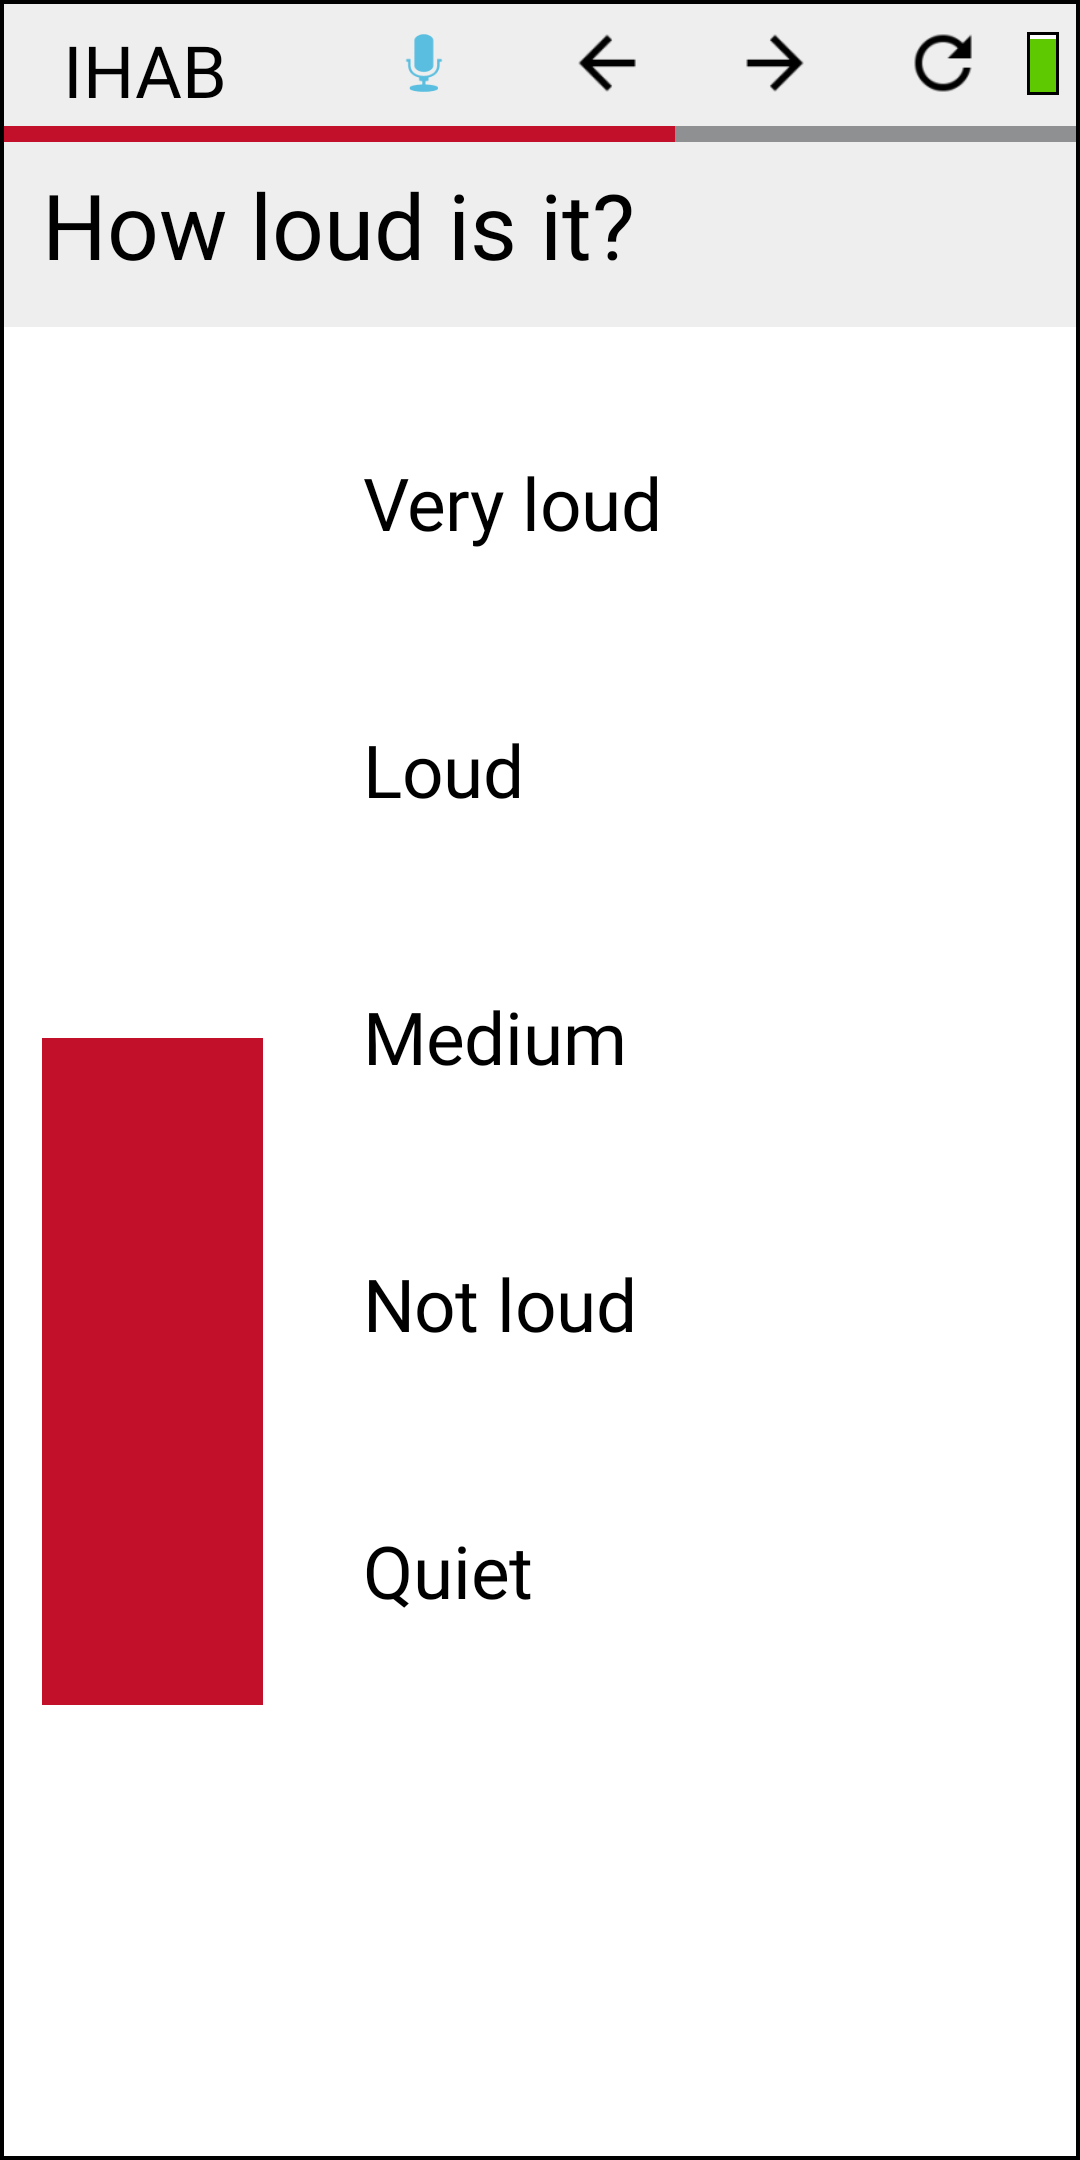
\includegraphics[width=0.30\textwidth]{images/screen_sliderfix_box.png}
		}
	\end{tabular}\\
\end{center}


\subsubsection{Free Slider}

Free sliders are fully functional sliders which allow the user to select any value on a given scale. The result is coded as a floating point value between 0 and 1.

\begin{center}
\hspace{-1.1cm}
	\begin{tabular}{p{0.68\textwidth} p{0.25\textwidth}} 
		\raisebox{-\totalheight}{
		\begin{tcolorbox}[colback=black!10!white,colframe=black!50!white, boxsep=1pt,left=4pt,right=4pt,top=4pt,bottom=2pt]
		\texttt{\noindent
			$<$question id="10106" type="sliderFree"$>$\newline
			\hspace*{0.5cm}$<$label$>$\newline
			\hspace*{1.0cm}$<$text>How loud is it?$<$/text$>$\newline
			\hspace*{0.5cm}$<$/label$>$\newline
			\hspace*{0.5cm}$<$option id="10106\_01"$>$\newline
			\hspace*{1.0cm}$<$text$>$Very loud$<$/text$>$\newline
			\hspace*{0.5cm}$<$/option$>$\newline
			\hspace*{0.5cm}$<$option id="10106\_02"$>$\newline
			\hspace*{1.0cm}$<$text>Loud$<$/text$>$\newline
			\hspace*{0.5cm}$<$/option$>$\newline
			\hspace*{0.5cm}$<$option id="10106\_03"$>$\newline
			\hspace*{1.0cm}$<$text>Medium$<$/text$>$\newline
			\hspace*{0.5cm}$<$/option$>$\newline
			\hspace*{0.5cm}$<$option id="10106\_04"$>$\newline
			\hspace*{1.0cm}$<$text$>$Not loud$<$/text$>$\newline
			\hspace*{0.5cm}$<$/option$>$\newline
			\hspace*{0.5cm}$<$option id="10106\_05"$>$\newline
			\hspace*{1.0cm}$<$text>Quiet$<$/text$>$\newline
			\hspace*{0.5cm}$<$/option$>$\newline
			$<$/question$>$
			}
		\end{tcolorbox} 
		}
		&
		\vspace{-0.29cm}
		\raisebox{-\totalheight}{
			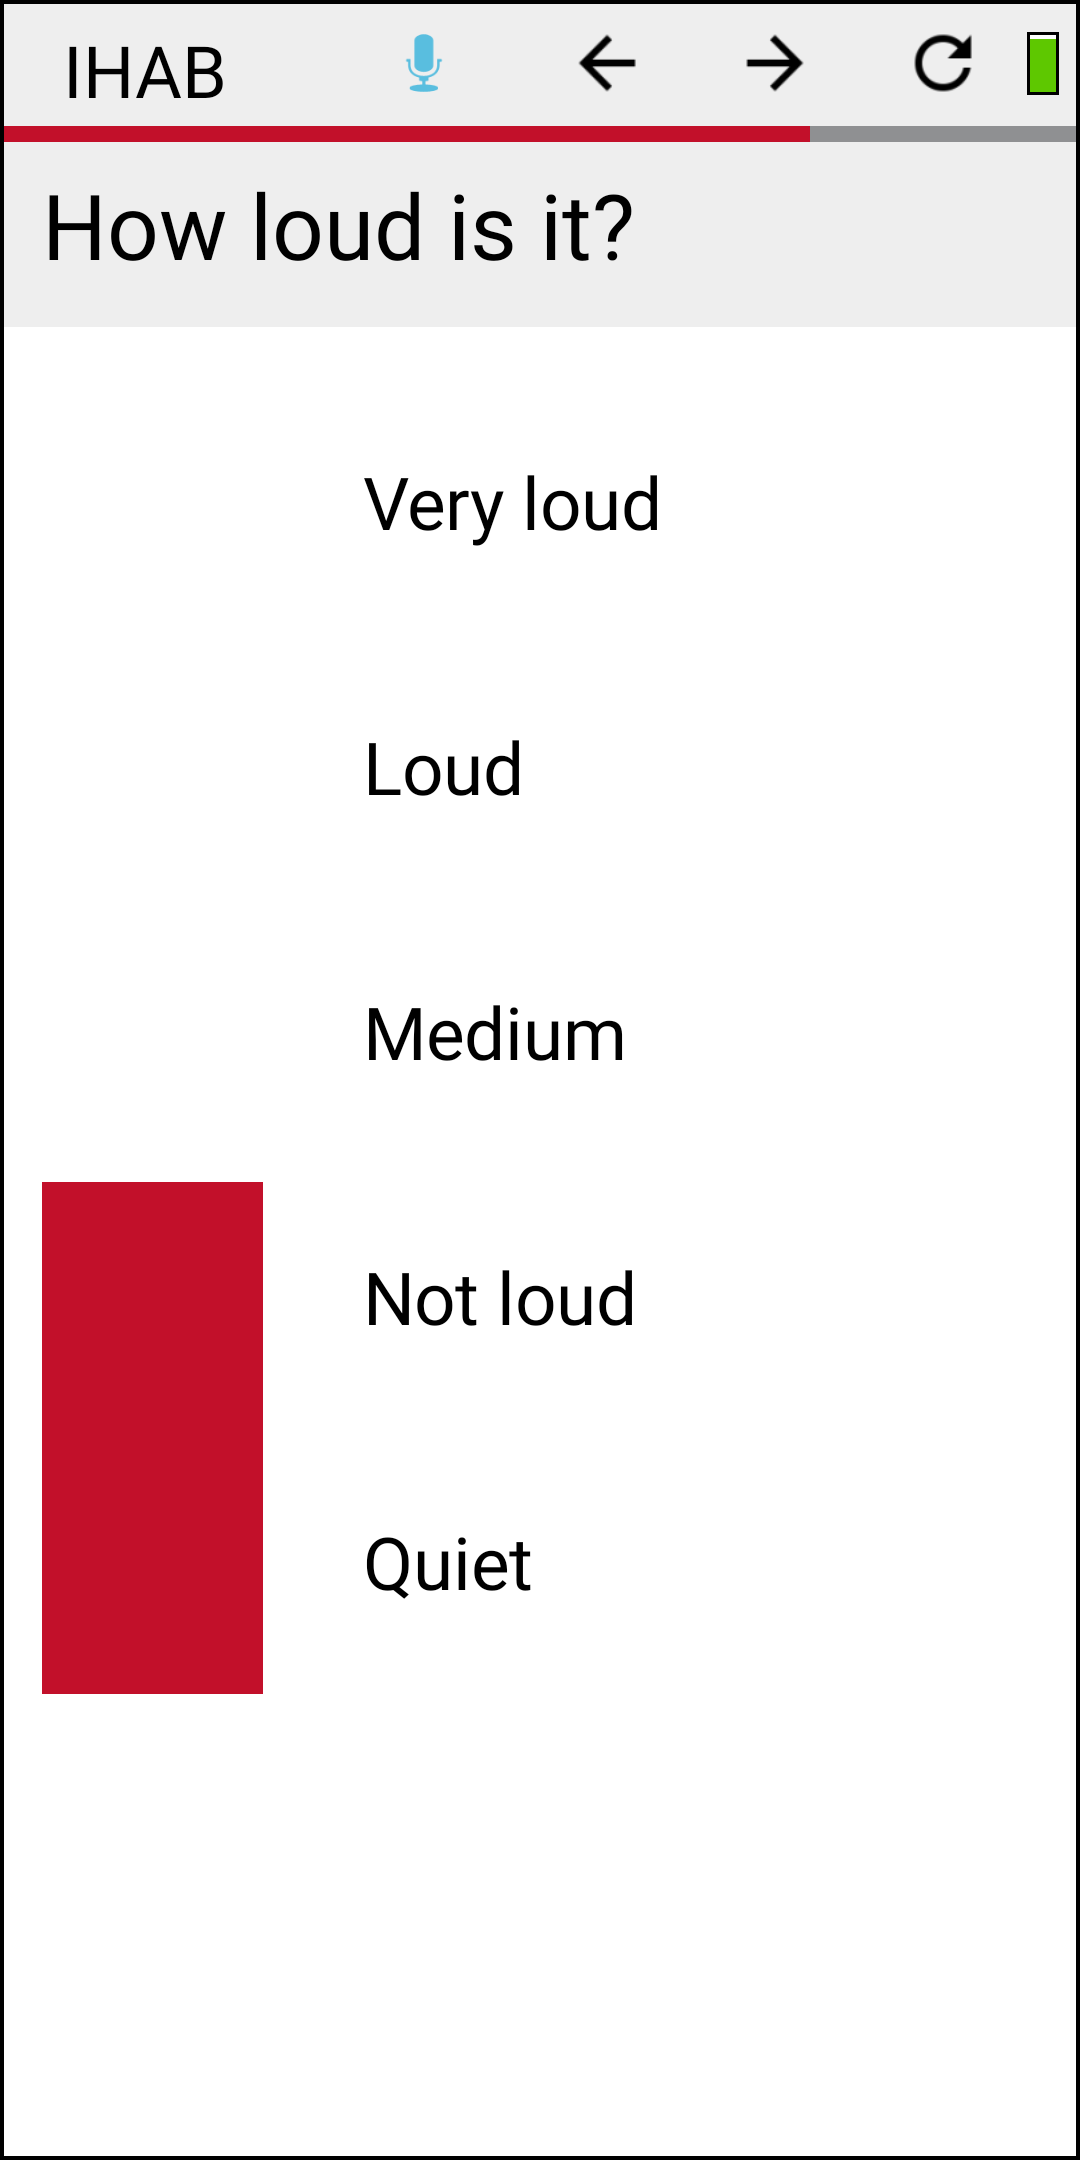
\includegraphics[width=0.30\textwidth]{images/screen_sliderfree_box.png}
		}
	\end{tabular}\\
\end{center}


\subsubsection{External Website}

As the name suggests, it is possible to include one or more external websites in the questionnaire, as long as internet access is provided. Two methods of calling exist. Either a website is linked without any additional information or with an identifier submitted to the server running the website. This can be helpful when the purpose of the external contents is to complete a supplementary task the results of which need to be associated with the user later. In this case a server would of course be expecting additional information of a certain format, and the term \$clientID\$ is internally replaced by the appropriate entry which is assigned via the preferences menu (\textit{Client ID}). Always ensure that the contents of the website is designed for display on a mobile device.

\begin{center}
\hspace{-1.1cm}
	\begin{tabular}{p{0.68\textwidth} p{0.25\textwidth}} 
		\raisebox{-\totalheight}{
		\begin{tcolorbox}[colback=black!10!white,colframe=black!50!white, boxsep=1pt,left=4pt,right=4pt,top=4pt,bottom=2pt]
		
		\textbf{Simple call:}\\
		
		\texttt{\noindent
			$<$question id="10107" type="website"$>$\newline
			\hspace*{0.5cm}$<$label$>$\newline
			\hspace*{1.0cm}$<$text>External Source:$<$/text$>$\newline
			\hspace*{0.5cm}$<$/label$>$\newline
			\hspace*{0.5cm}$<$option id="10107\_01"$>$\newline
      \hspace*{1.0cm}$<$text$>$https://tgm.jade-hs.de/projekte/\newline
			\hspace*{2.0cm}ihab-rl$<$/text$>$\newline
			\hspace*{0.5cm}$<$/option$>$\newline
			$<$/question$>$\\
			}
			
			\textbf{Call with parameter:}\\
		
		\texttt{\noindent
			$<$question id="10108" type="website"$>$\newline
			\hspace*{0.5cm}$<$label$>$\newline
			\hspace*{1.0cm}$<$text>External Source:$<$/text$>$\newline
			\hspace*{0.5cm}$<$/label$>$\newline
			\hspace*{0.5cm}$<$option id="10108\_01"$>$\newline
      \hspace*{1.0cm}$<$text$>$https://tgm.jade-hs.de/projekte/\newline
			\hspace*{2.0cm}ihab-rl/index.php?ClientId=\$clientID\$\newline
			\hspace*{1.0cm}$<$/text$>$\newline
			\hspace*{0.5cm}$<$/option$>$\newline
			$<$/question$>$
			}
		\end{tcolorbox} 
		}
		&
		\vspace{-0.29cm}
		\raisebox{-\totalheight}{
			
\includegraphics[width=0.3\textwidth]{images/screen_website_box.png}
		}
	\end{tabular}\\
\end{center}


\subsubsection{Finish}

The last question must be the finish page which automatically includes a button that completes the questionnaire and saves the results:

\begin{center}
\hspace{-1.1cm}
	\begin{tabular}{p{0.68\textwidth} p{0.25\textwidth}} 
		\raisebox{-\totalheight}{
			\begin{tcolorbox}[colback=black!10!white,colframe=black!50!white, boxsep=1pt,left=4pt,right=4pt,top=4pt,bottom=2pt]
				\texttt{\noindent
				$<$finish$>$\\
				\hspace*{0.5cm}$<$text$>$Thank you!$<$/text$>$\\
				$<$/finish$>$
				}
			\end{tcolorbox} 
		}
	&
		\vspace{-0.29cm}
		\raisebox{-\totalheight}{
			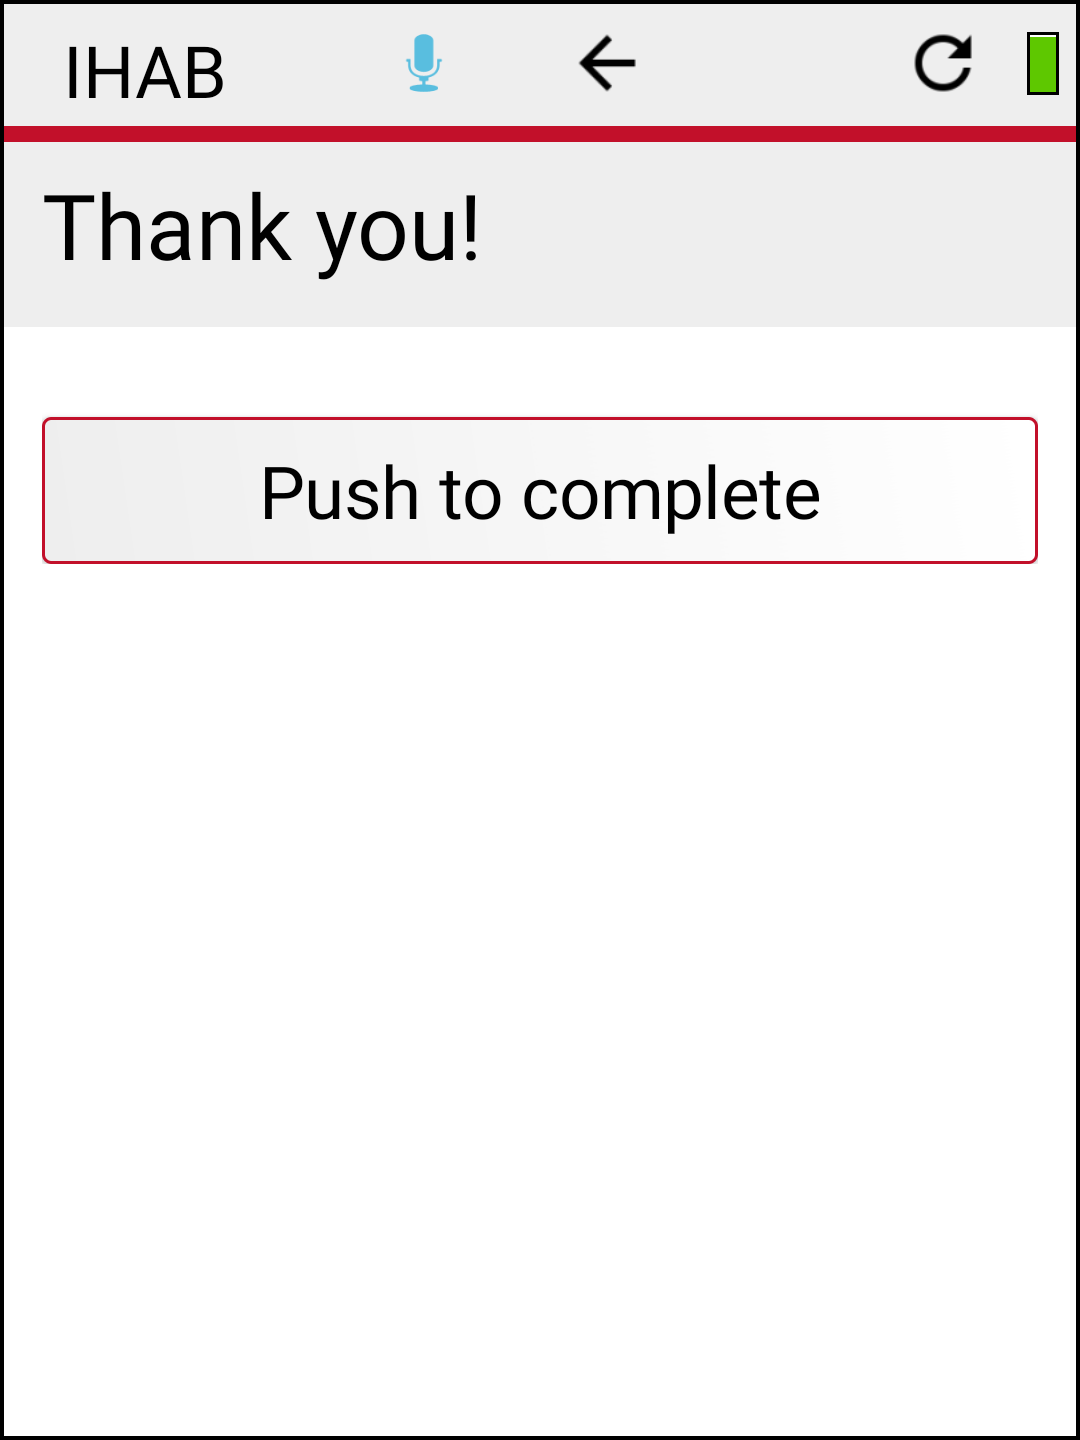
\includegraphics[width=0.30\textwidth]{images/screen_finish_crop_box.png}
		}
	\end{tabular}\\
\end{center}


\subsection{Checkbox grouping and exclusivity}\label{subsec:goupingandexclusivity}

If only one option out of a group of options might be logically possible (see exemplary options 1-3 below), they can form a \texttt{group}. If one item out of this group is selected, the others are automatically deselected. Multiple groups can exist within one question. An extreme form of this is the \texttt{exclusive} tag (option 5), which deselects every other item from the respective list of answers except itself and automatically deselects itself if another item is chosen.

\begin{center}
	\begin{tcolorbox}[colback=black!10!white,colframe=black!50!white, boxsep=1pt,left=4pt,right=4pt,top=4pt,bottom=2pt]
		\texttt{\noindent
			$<$question id="10111" type="checkbox"$>$\\
			\hspace*{0.5cm}$<$label$>$\\
			\hspace*{1cm}$<$text$>$Where does sound originate from?$<$/text$>$\\
			\hspace*{0.5cm}$<$/label$>$\\
			\hspace*{0.5cm}$<$option id="10111\_01" group="1"$>$\\
			\hspace*{1cm}$<$text$>$Single person$<$/text$>$\\
			\hspace*{0.5cm}$<$/option$>$\\
			\hspace*{0.5cm}$<$option id="10111\_02" group="1"$>$\\
			\hspace*{1cm}$<$text$>$2-3 persons$<$/text$>$\\
			\hspace*{0.5cm}$<$/option$>$\\
			\hspace*{0.5cm}$<$option id="10111\_03" group="1"$>$\\
			\hspace*{1cm}$<$text$>$4 or more persons$<$/text$>$\\
			\hspace*{0.5cm}$<$/option$>$\\
			\hspace*{0.5cm}$<$option id="10111\_04"$>$\\
			\hspace*{1cm}$<$text$>$Public announcement$<$/text$>$\\
			\hspace*{0.5cm}$<$/option$>$\\
			\hspace*{0.5cm}$<$option id="10111\_05" condition="exclusive"$>$\\
			\hspace*{1cm}$<$text$>$It is quiet.$<$/text$>$\\
			\hspace*{0.5cm}$<$/option$>$\\
			$<$/question$>$
		}
	\end{tcolorbox}
\end{center}


\subsection{Default items}

An item can be preselected by default using the \texttt{default} tag instead of \texttt{option} as shown below. This is supported by radio buttons, checkboxes, emojis, and sliders.

\begin{center}
	\begin{tcolorbox}[colback=black!10!white,colframe=black!50!white, boxsep=1pt,left=4pt,right=4pt,top=4pt,bottom=2pt]
		\texttt{\noindent
			$<$default id="10102\_02"$>$\\
			\hspace*{0.5cm}$<$text$>$Green$<$/text$>$\\
			$<$/default$>$
		}
	\end{tcolorbox}
\end{center}


\subsection{Forced answers}

Sometimes a question might be very important and a missing answer is not an option. In this case the command \texttt{forceAnswer="true"} comes in handy. The user is unable to skip the question and after 3 attempts a dialog box with a reminding message appears on the screen.

\begin{center}
\hspace{-1.1cm}
	\begin{tabular}{p{0.68\textwidth} p{0.25\textwidth}} 
		\raisebox{-\totalheight}{
			\begin{tcolorbox}[colback=black!10!white,colframe=black!50!white, boxsep=1pt,left=4pt,right=4pt,top=4pt,bottom=2pt]
		\texttt{\noindent
			$<$question id="10101"\newline
			\hspace*{0.5cm}type="radio" \newline
			\hspace*{0.5cm}forceAnwer="true"$>$
		}
	\end{tcolorbox}
		}
	&
		\vspace{-0.29cm}
		\raisebox{-\totalheight}{
			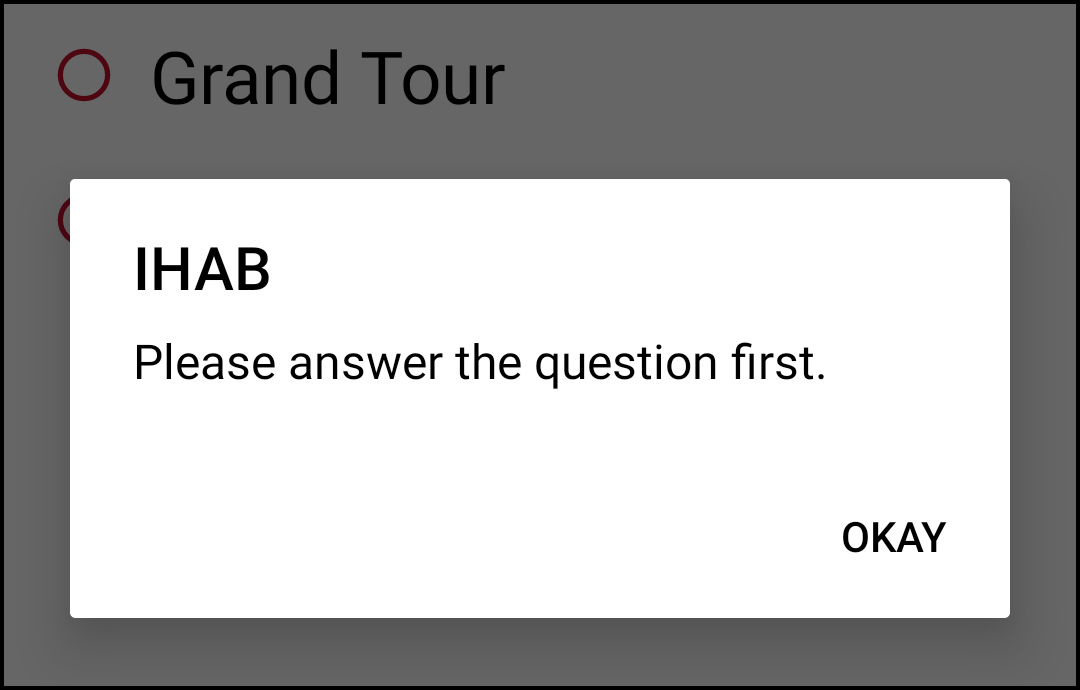
\includegraphics[width=0.30\textwidth]{images/screen_force_box_crop.png}
		}
	\end{tabular}\\
\end{center}


\subsection{Logic}\label{sub:logic}

In order to allow for high specificity and efficiency, questions can be equipped with logical decision parameters that establish whether or not a question will be included in the current suite. The switch is located in the opening line of each question under the tag \texttt{filter} in form of a comma-separated concatenation of all included conditions.\\
\\
Two scenarios exist: positive and negative. A question will only be included if \textbf{ALL} positive conditions are satisfied and it will not be included as soon as at least \textbf{ONE} negative condition (indicated by a prefixed ``!'') is satisfied (e.g. \texttt{filter="10103\_02,10103\_05,!10111\_09"}).\\ 
\\
$\rightarrow$ Think: positive - necessary criterion, negative -- sufficient criterion.\\
\\
The filter conditions are the option ID's of answer items from earlier questions of the current session. Whenever an answer is chosen by the user, its ID is stored in memory and before a question is displayed, a filter checks whether given conditional ID's are present in the memory.\\

\begin{center}
	\begin{tcolorbox}[colback=black!10!white,colframe=black!50!white, boxsep=1pt,left=4pt,right=4pt,top=4pt,bottom=2pt]
		\texttt{\noindent
			$<$question id="10112" type="radio" filter="10103\_02,10103\_05,!10111\_09"$>$
		}
	\end{tcolorbox}
\end{center}

Note that entries can be spread across multiple lines in order to increase readability.

\begin{center}
	\begin{tcolorbox}[colback=black!10!white,colframe=black!50!white, boxsep=1pt,left=4pt,right=4pt,top=4pt,bottom=2pt]
		\texttt{\noindent
			$<$question id="10112"\newline
			\hspace*{0.5cm}type="radio" \newline
			\hspace*{0.5cm}filter="10103\_02,\newline
			\hspace*{1.0cm}10103\_05,\newline
			\hspace*{1.0cm}!10111\_09"$>$
		}
	\end{tcolorbox}
\end{center}


\subsection{Comments}

Two types of comments are supported by the questionnaire format. Single line comments start with ``//'', comments spread across multiple lines are parenthesized by ``\texttt{$/*$}'' and ``\texttt{$*/$}''.

\begin{center}
	\begin{tcolorbox}[colback=black!10!white,colframe=black!50!white, boxsep=1pt,left=4pt,right=4pt,top=4pt,bottom=2pt]
		\texttt{\noindent
			// One line comment\newline
			\newline
			/* Here is a\newline
			slightly longer\newline
			comment */
		}
	\end{tcolorbox}
\end{center}



\clearpage


\section{Resulting file}

Completing a questionnaire results in an .xml file being generated in the ``data'' folder. The file name is composed of the Device ID, the current date in \texttt{yyyyMMdd} (year, month, day) and the time of completion in \texttt{HHmmssSSS} (24h hours, minutes, seconds, milliseconds), for example \texttt{cbaaacf404279a80\_20200430\_125224699.xml}.\\
\\
The file contains information on whether the questionnaire was taken upon a reminder or deliberately (\texttt{motivation}: auto/manual), which questionnaire design it was based on, the Device ID, version of the application, start and end dates as well as the provided answers.

\begin{center}
	\begin{tcolorbox}[colback=black!10!white,colframe=black!50!white, boxsep=1pt,left=4pt,right=4pt,top=4pt,bottom=2pt]
		\texttt{\noindent
			$<$?xml version="1.0" encoding="utf-8"?$>$\newline
			$<$mobiquest$>$\newline
			$<$motivation motivation ="manual"/$>$\newline
			$<$record uri="tmp/cbaaacf404279a80\_20200430\_125224699.xml"\newline
			\hspace*{0.5cm}survey\_uri="tmp.xml"$>$\newline
			$<$value device\_id="cbaaacf404279a80"/$>$\newline
			$<$value start\_date="2020-04-30T12:52:24"/$>$\newline
			$<$value start\_date\_UTC="2020-04-30T12:52:24"/$>$\newline
			$<$value app\_version="1.5"/$>$\newline
			$<$value question\_id="10101" option\_ids="1010102"/$>$\newline
			$<$value question\_id="10102" option\_ids="1010202"/$>$\newline
			$<$value question\_id="10103" option\_ids="1010301"/$>$\newline
			$<$value question\_id="10104" option\_ids="Some generic text."/$>$\newline
			$<$value question\_id="10105" option\_ids="1010504"/$>$\newline
			$<$value question\_id="10106" option\_ids="0.36958176"/$>$\newline
			$<$value question\_id="10107"/$>$\newline
			$<$value end\_date="2020-04-30T12:53:13"/$>$\newline
			$<$value end\_date\_UTC="2020-04-30T12:53:13"/$>$\newline
			$<$/record$>$\newline
			$<$/mobiquest$>$
		}
	\end{tcolorbox}
\end{center}


\clearpage


\section{Objective data}

Additional to the facilitation of questionnaires, the IHAB application also offers real-time extraction of acoustic features, based on the operation mode (see \ref{sub:operationmode}). These features are namely \emph{RMS Level}, \emph{Zero-Crossing-Rate} (ZCR), and \emph{Power Spectral Density} (PSD) and they are stored in chunks of a size that can be edited inside the preferences menu (usually a length of 60\,s). Although we recommend data extraction and interpretation using our Matlab interface (see \ref{sec:transfer}), here is some information on the file structure, which holds true for every feature. Each file contains a header which is holding basic information e.g. time stamps, sampling rate, dimensions, and logistics like frame length or hop size. The header is followed by a series of data packages that follow the structure depicted below.\\

\textbf{Header:}

\begin{center}
	\begin{tcolorbox}[colback=black!10!white,colframe=black!50!white, boxsep=1pt,left=4pt,right=4pt,top=4pt,bottom=2pt]
	\texttt{
		\begin{tabularx}{\textwidth}{l|l|X} 
			Type & \# & Contents\\
			\hline
			int32 & 1 & \# frames in current chunk\\
			int32 & 1 & \# dimensions (including frame time stamps)\\
			int32 & 1 & block size in samples\\
			int32 & 1 & hop size in samples\\  
			int32 & 1 & audio sampling rate\\
			byte & 16 & time stamp of block (yyyyMMdd\_HHmmssSSS)\\
		\end{tabularx}
		}
	\end{tcolorbox}
\end{center}

\textbf{Data:}

\begin{center}
	\begin{tcolorbox}[colback=black!10!white,colframe=black!50!white, boxsep=1pt,left=4pt,right=4pt,top=4pt,bottom=2pt]
	\texttt{
		\begin{tabularx}{\textwidth}{l|l|X} 
			Type & \# & Contents\\
			\hline
			double & N & block time + data\\
		\end{tabularx}
		}
	\end{tcolorbox}
\end{center}

N is the number of dimensions including timestamps times the number of blocks or frames inside a chunk. Times and feature data are concatenated as follows with block times respectively denoting beginning and end of a block:\\

\begin{tcolorbox}[colback=black!10!white,colframe=black!50!white, boxsep=1pt,left=4pt,right=4pt,top=4pt,bottom=2pt]
	\texttt{
		[ blocktime(1) blocktime(2) feature(1) feature(2) ... feature(L-2)\\
		\color{black!10!white}[\ \ \color{black} blocktime(2) blocktime(3) feature(1) feature(2) ... feature(L-2) ]
	}
\end{tcolorbox}
\vspace{0.5cm}
with L being the block size in samples and the data formatted as big endian.


\clearpage


\section{Data transfer}\label{sec:transfer}

For every questionnaire that has been answered, a resulting .xml file is produced which can be found in the \textit{data} folder within the application directory. In order to simplify data transfer we have developed a Matlab interface which can also be used to stop the application (because for safety reasons this is not provided or at least not trivial) and to erase all data from the device. The software is self-explanatory and can be found under GitHub: \url{https://github.com/IHAB-RL/IHAB_DataExtraction.git}. Please note that so far it has only been tested under Windows 7/10.

\begin{figure}[h]
	\centering
		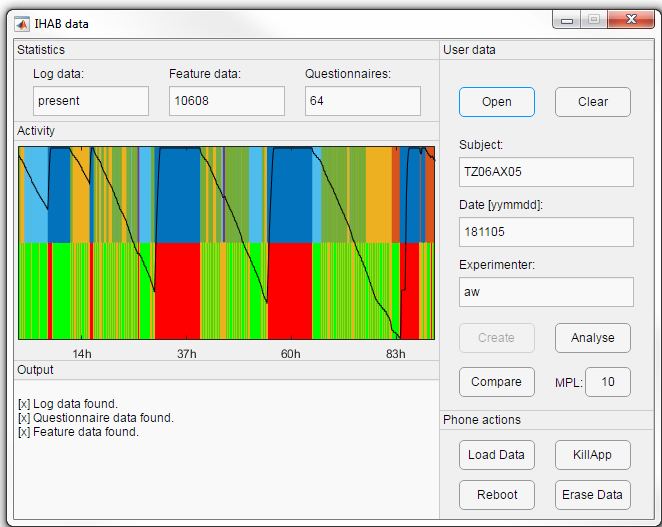
\includegraphics[width=0.90\textwidth]{images/DataExtractor.png}
	\label{fig:DataExtractor}
\end{figure}


\clearpage


\section{License}

 Copyright 2020 \Institute\\
\\
   Licensed under the Apache License, Version 2.0 (the ``License'');
   you may not use this file except in compliance with the License.
   You may obtain a copy of the License at\\
\\
	 \url{http://www.apache.org/licenses/LICENSE-2.0}\\
\\
   Unless required by applicable law or agreed to in writing, software
   distributed under the License is distributed on an ``AS IS'' BASIS,
   WITHOUT WARRANTIES OR CONDITIONS OF ANY KIND, either express or implied.
   See the License for the specific language governing permissions and
   limitations under the License.

\end{document} 